\chapter{Justificación Teórica}
\section{Introducción}
%https://www.thetechedvocate.org/8-ways-machine-learning-will-improve-education/
La planificación de grupos no se entiende sin tener en cuenta el uso de la predicción. Para poder planificar el numero de grupos para el nuevo curso, se debe tener en cuenta los datos del curso previo; es a partir de estos datos con los que se realiza un analisis predictivo.

Uno de los intereses que se tienen a la hora de realizar cualquier proyecto de análisis de datos, ``Big Data'', ``Business Intelligence'' o análisis predictivo son las variables a utilizar, ya que son las que permiten obtener la mayoría de información.

Esta investigación se realiza con el propósito de aportar conocimiento existente sobre la importancia de determinadas variables, metodologías, modelos y la relevancia de estos últimos en la predicción, la planificación y la gestión educativa, concretamente en la previsión de la sobrepoblación en el aula. 

Para ello, y, teniendo en cuenta los propósitos de esta investigación, se debe establecer el objeto de búsqueda de documentación científica acerca de la minería de datos en el ámbito educativo, más concretamente, en la educación secundaria. 

A partir del objeto de búsqueda, se debe establecer las fuentes que se utilizan para obtener resultados fiables, ya que en la actualidad existen numerosos artículos acerca del uso de la ciencia de datos, pero es necesario acotar la búsqueda a lo relativo a educación.

Debemos destacar que la mayoría de los resultados obtenidos tratan de artículos centrados en la predicción de los resultados académicos de los alumnos teniendo en cuenta ciertos factores internos (como las propias calificaciones a lo largo del curso) y externos (como factores etnográficos, edad, situación económica familiar, etc.). Estos factores se utilizan principalmente para obtener una aproximación sobre las calificaciones, y el fracaso escolar. Mostrando de forma implícita las relaciones de estos aspectos con el resultado (calificación).

\section{Análisis trabajos previos relevantes}
En este apartado se resaltan los artículos más representativos que realizan un estado del arte sobre la minería de datos en la educación, recogiendo información genérica de otros artículos.  Estos artículos más representativos sirven de referencia no sólo para obtener nuevos artículos sino para ver las metodologías comunes utilizadas y las aplicaciones concretas de la ciencia de datos en el ámbito educativo.

En este sentido se pueden destacar los artículos de \citeA{inbook}, \citeA{romero2010educational} y \citeA{PENAAYALA20141432}.

\citeA{inbook} en su artículo, realizan una revisión sobre las publicaciones realizadas, citando diversos artículos y resumiendo brevemente el estudio y las técnicas y algoritmos utilizadas en este. Además, de forma genérica agrupa los algoritmos más utilizados en las técnicas de clasificación, ``clustering'' y regresión.

En el artículo de \citeA{PENAAYALA20141432} se muestra el número de publicaciones existentes hasta el momento que utilizan ciertos algoritmos predictivos como el K-Means, J-48, Naives Bayes, etc. En este mismo artículo, se clasifican las publicaciones en seis categorías. Podemos destacar que la categoría mayoritaria (con un 21\%) es el modelado del comportamiento del alumno seguida del rendimiento académico del alumno (con un 20\%). \citeA{romero2010educational} utiliza también categorías para clasificar las publicaciones.

Mediante estos artículos se ha obtenido una vista general de la minería de datos, proporcionando información y realizando comparaciones que acotan la búsqueda de nuevas técnicas, herramientas, algoritmos, etc.

%LOS MAS GENÉRICOS SON EN ESTE PUNTO, HAY QUE ACLARARLO. CON ALGUNA FRASE

\section{Estudios más relacionados con la minería de datos en educación}
%Después de realizar un análisis sobre los artículos encontrados, se ha descubierto que la minería de datos se utiliza para resolver distintos problemas en la educación.
Este apartado se centra en las categorías -comentadas anteriormente- que tienen mayor relación con el problema a resolver en este tipo de investigación. %De esta forma se puede observar como dichos artículos satisfacen con sus propios objetivos.

Teniendo en cuenta esta serie de clasificaciones o categorías sobre las publicaciones realizadas sobre minería de datos en la educación. La mayoría de los artículos se centran en el rendimiento y en las calificaciones de los alumnos y, cómo teniendo en cuenta estas investigaciones, se puede mejorar la calidad educativa.

En el artículo de \citeA{FERNANDES2019335}, los datos escolares a estudiar proceden de alumnos de colegios de un Distrito Federal de Brasil durante el 2015 y el 2016. Estos datos se obtienen a partir de la base de datos de iEducar que contiene atributos relacionados con cada alumno. 

Algunas de las variables que se estudian en este artículo pertenecen concretamente al ámbito personal, social y geográfico del alumno. Estas variables son: el barrio del alumno, el centro educativo, la edad del alumno, los ingresos del alumno, los alumnos con necesidades especiales, el género y el entorno en el aula.

Como conclusiones, se indica en este artículo que el entorno social y sus variables tienen una influencia directa en el proceso de enseñar-aprender. %Esta investigación puede aportar información a los profesionales que busquen herramientas o métodos para mejorar los resultados escolares de los alumnos.

Por otro lado, en el artículo de \citeA{ASIF2017177}, se realizan otras investigaciones relativas al rendimiento académico, donde también se utilizan variables sociales como la edad, sexo, nacionalidad, estado civil, desplazamiento (si el alumno vive fuera del distrito), necesidades especiales, tipo de admisión, situación laboral, situación económica, etc.

%Los datos utilizados en este artículo proceden de las calificaciones del cuarto año del grado de ingeniería de Tecnología Informática de una universidad de Pakistán. Se van a tomar 210 alumnos que se han matriculado en los cursos de 2007-2008 y 2008-2009. Los datos contienen variables relacionadas con las calificaciones de pre-admisión de los alumnos y de las calificaciones de estos en los siguientes 4 años del programa de grado.

El objetivo es, nuevamente, obtener información sobre el rendimiento de estudiantes para que las personas interesadas (directores y docentes) puedan mejorar el programa educativo. %Los enfoques para lograr este objetivo son los siguientes:

Otro de los artículos que se ha utilizado como referencia ha sido el de \citeA{SHAHIRI2015414}. En este artículo, nuevamente se utilizan técnicas predictivas para la mejora del rendimiento académico de los alumnos. En este caso, los datos utilizados proceden de instituciones malayas. De nuevo se tienen en cuenta los resultados académicos internos como las calificaciones de prácticas o tareas, exámenes, actividades en el laboratorio, test de clase y atención. También se ha tenido en cuenta factores externos como el género, la edad, el entorno familiar y la discapacidad. 

Relacionado con el rendimiento académico, existe también un artículo en el que se realiza labores de predicción para evitar el fracaso escolar. En este artículo, \cite{vera2012prediccion}, se seleccionan variables en el que se incluyen si el alumno fuma, bebe, si tiene alguna discapacidad física, la edad, el nivel económico entre otras muchas. Los datos de este artículo se obtienen a partir de encuestas realizadas a alumnos del Centro Nacional de Evaluación y del Departamento de Servicios Escolares. Relacionado también con el rendimiento académico, esta el artículo de \citeA{kaur2015classification} donde se utilizan variables como el uso del móvil por parte del alumno, el tipo del colegio, la localización de este (áreas urbanas o rurales), el acceso a Internet del alumno, etc. Siendo las variables de la existencia de Internet y ordenador en casa las que más afectan en la predicción. En este estudio, la variable a predecir en esta investigación es si el alumno se gradúa o no.

Se ha encontrado un artículo referente a la educación en España, este artículo es el de \citeA{jose2016explotacion}, en el que se analiza las calificaciones y las tareas para cada trimestre de estudiantes de Bachillerato y ESA (Educación Secundaria para Adultos). \citeauthor{jose2016explotacion} en este artículo, se utilizan datos de alumnos de un determinado centro público de Andalucía. Los cursos de alumnos que evalúa son 1º y 2º de Bachillerato y de ESA. 

También se ha revisado un artículo relacionado con la mejora académica de alumnos de ingeniería en los primeros 3 años de titulación. Este artículo de \citeA{ADEKITAN2019e01250} utiliza datos de una universidad de Nigeria. 
%Este articulo realiza una exploración sobre 1841 estudiantes durante sus primeros 3 años, entre los años 2002 y 2014. 
Inicialmente se consideraron 18 variables, sin embargo, solo se utilizaron 6 variables que son las siguientes: matriculación, genero, especialidad de los estudiantes, ciudad del estudiante, calificaciones y tipo de educación secundaria recibida previamente.

En el artículo de \citeA{alvarez2010violencia} se analiza la relación entre la violencia y la repetición de curso. En la investigación realiza un cuestionario a 1742 estudiantes de 7 centros. Según el artículo, los resultados obtenidos indican que la violencia es mayor cuando los alumnos repiten de curso. Alguna de las variables que se estudian son: violencia de profesorado hacia alumnado, violencia física indirecta por parte del alumnado, violencia verbal de alumnado hacia alumnado, violencia física directa entre alumnado y violencia verbal de alumnado hacia profesorado.

En el libro de \citeA{PANAHI2019161}, se ha realizado una serie de investigaciones cuyo objetivo ha sido determinar la idoneidad de construir o emplazar centros educativos según pesos dados a factores. Estos factores son los siguientes:

\begin{itemize}
	\item \textbf{Facilidades Urbanas:} En este punto se incluyen las gasolineras, las tuberías de gas de alta presión y las líneas de alta tensión. Cuanto más cerca estén los centros de estas zonas, más riesgo existe para los alumnos. Se tiende por tanto a alejar los centros de estos puntos.
	\item \textbf{Densidad de población y áreas residenciales:} La proximidad de los colegios a zonas residenciales con una gran población de estudiantes es importante, puesto que, a menor distancia entre los estudiantes, los colegios y sus casas menor es el gasto de las familias y menor es la probabilidad de que los alumnos sean secuestrados.
	\item\textbf{ Accesibilidad a red de carreteras urbanas:} La distancia de las calles y las autovías es otro factor importante para situar los colegios. Cuanto más cerca estén los colegios a estas vías, más facilidades tendrán los alumnos, y por lo tanto más ahorro de tiempo y costes.
	Sin embargo, la cercanía de los colegios a las autovías o autopistas, puede implicar mayor riesgo de accidentes. Sin embargo, si las autovías o autopistas se encuentran lejos, se reduce la accesibilidad a los colegios. Es necesario situar los centros en puntos intermedios (100-200m).
	\item \textbf{Servicios Urbanos:} Las distancias a los hospitales, a las estaciones de bomberos y de policía tienen mayor influencia. Sin embargo, estos deben situarse a distancias prudenciales de los centros (100-200m).
	\item \textbf{Centros culturales:} La proximidad de los centros culturales incrementa la salud espiritual y psicológica del alumno, incrementando así sus conocimientos. Curiosamente, si existen estos tipos de centros cercanos al colegio, entonces no es necesario que dichos colegios dispongan de estos servicios (pudiéndose ampliar las aulas, el comedor, etc)
\end{itemize}                     

La investigación se lleva a cabo en la ciudad de Tehran. Se han tomado para el estudio dos distritos. Uno de ellos contiene 106 colegios y el otro 137. A partir de la geolocalización de dichos colegios y de los sub-factores comentados, se ha realizado un estudio sobre la relación existente entre los factores, sub-factores y los colegios.

%Los pesos dados a cada factor y sub-factor se han determinado utilizando un algoritmo llamado SWARA. 
El objetivo de este articulo es determinar la idoneidad para seleccionar los lugares de construcción de los centros, investigando los sub-factores dados.

Los resultados finales que se obtienen indican que los factores por orden de importancia para la construcción son: los posibles daños que puedan amenazar a los alumnos y sus familias, la reducción del coste para las familias y el incremento de la eficiencia escolar.

\section{Metodología de trabajo en el desarrollo de proyectos de minería de datos}
En primer lugar, y antes de realizar cualquier trabajo, es necesario tener en cuenta una metodología valida a seguir, es decir, se debe seguir una serie de pasos para conseguir los objetivos determinados. Por tanto, en este apartado se va a estudiar los métodos de trabajo existentes en los artículos estudiados, ver sus ventajas y desventajas para posteriormente seleccionar el que se considere apto para esta investigación.

Existen distintas metodologías de trabajo para realizar un proyecto de minería de datos. Sin embargo, según el artículo de \citeA{moine2011analisis}, las metodologías que abarcan todas las posibles etapas de un proyecto serían las metodologías CRISP-DM y Catalyst. El resto de metodologías no completan todas las fases que se debe o simplemente establecen los pasos a seguir, pero no las tareas. La comparativa se muestra en la figura \ref{fig:compMod}.

\begin{figure*}[htb]
	\centering
	\caption{
		Comparación de metodologías de Minería de Datos. Recuperado de \protect\citeA{moine2011analisis}
	}
	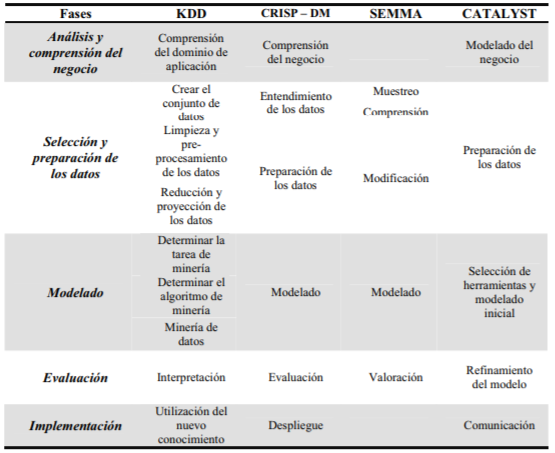
\includegraphics[width=0.8\textwidth]{recursos/ComparacionModelosDM}
	\label{fig:compMod}
\end{figure*}
\FloatBarrier


La metodología de trabajo predominante en los artículos observados de carácter educativo ha sido la metodología CRISP-DM (del inglés Cross Industry Standard Process for Data Mining) que es una metodología frecuente en el desarrollo de proyectos de minería de datos. Esta metodología indica cómo debe realizarse, mediante tareas, dichos proyectos. Esta metodología se ha utilizado en artículos como \citeA{FERNANDES2019335}, \citeA{DELEN2010498}, \citeA{SEN20129468}, \citeA{jaramillo2015aplicacion} y \citeA{chalaris2014improving}.

Según \citeA{jaramillo2015aplicacion}, en su investigación se ha seleccionado Crisp-DM por las siguientes razones: ''La metodología a utilizar es Crisp-DM ya que cada una de sus fases se encuentra claramente estructurada definiendo de tal forma las actividades y tareas que se requieren para lograr el objetivo planteado, es decir, la más completa entre las metodologías comparadas, es flexible por ende se puede hacer usos de cualquier herramienta de minería de datos'', idea ya presentada en el artículo de \cite{moine2011analisis}.

\section{Modelos utilizados en el desarrollo de proyectos de minería de datos en el entorno educativo}
Una vez que se ha revisado los artículos existentes, se debe abstraer la información relativa a los modelos utilizados con el objetivo de obtener un estado de la situación de dichos modelos.

En el artículo de prensa de \citeA{FERNANDES2019335}, se muestra el uso de técnicas como los métodos de clasificación y el algoritmo predictivo de GBM (Gradient Boosting Model) con el objetivo de obtener aquellas variables en el entorno del alumnos que hacen que el modelo obtenga mejores o peores resultados escolares. Este estudio, además, tiene el objetivo de aportar información útil para los representantes políticos en el ámbito educativo, el consejo escolar y los profesores con el objetivo de que estos puedan realizar políticas públicas, materiales didácticos y trabajo social para beneficiar a los estudiantes.

En el artículo de \citeA{SHAHIRI2015414} se indica que ``a priori", sin tener en cuenta la experiencia, es necesario realizar un proyecto piloto, que responda a dos preguntas en concreto. La primera pregunta que se plantea son los atributos o variables a utilizar en la investigación. La segunda pregunta planteada es sobre los métodos predictivos a utilizar. La siguiente figura \ref{fig:precMet} obtenida del artículo, muestra la precisión en la predicción de los algoritmos entre los años 2002 y 2015.

\begin{figure*}[htb]
	\centering
	\caption{Predicción en la precisión agrupada por algoritmos desde 2002 a 2015. Recuperado de \protect\citeA{SHAHIRI2015414}}
	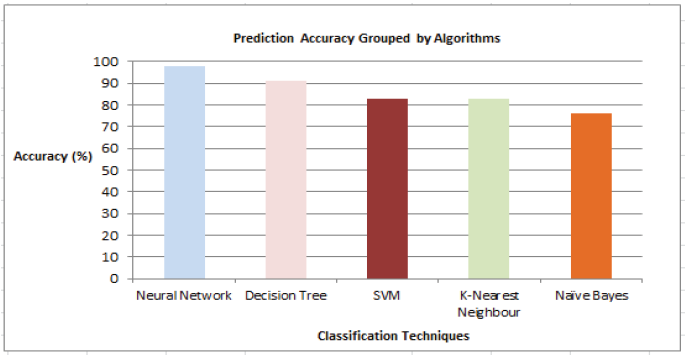
\includegraphics[width=0.8\textwidth]{recursos/PrecisionMetodos}
	\label{fig:precMet}
\end{figure*}

Teniendo en cuenta la figura \ref{fig:precMet}, se observa que las redes neuronales son las que obtienen mejores resultados junto con los arboles de decisiones, lo que significa que se ajustan más a los datos. 

Los resultados obtenidos en otro artículo, concretamente el de \citeA{ASHRAF20181021}, indican que el mejor modelo para los datos propuestos ha sido obtenido utilizando el algoritmo de bosques aleatorios. Este algoritmo ha obtenido mejores resultados que otros algoritmos como los arboles de decisión o árbol aleatorio. Este articulo utiliza también datos académicos de alumnos, en este caso, pertenecientes a la Universidad Kashmir.

Para lograr los objetivos establecidos en el análisis del rendimiento académico, \citeA{ASIF2017177}, va a utilizar los arboles de decisión, Naïves Bayes, Redes Neuronales, 1-Vecino-Cercano y Bosques Aleatorios. Los mejores resultados se han obtenido utilizando el algoritmo de Naïves Bayes, obteniendo un 85\% de precisión.

En cuanto al artículo de \citeA{ADEKITAN2019e01250}, nuevamente se utilizan algoritmos como redes neuronales, bosques aleatorios, arboles de decisión, Naïve Bayes, combinación de árboles y regresión logística. En la figura \ref{fig:compResMod} se puede observar la comparación entre los modelos.

\begin{figure*}[htb]
	\centering
	\caption{Comparación de los resultados obtenidos. Recuperado de \protect\citeA{ADEKITAN2019e01250}}
	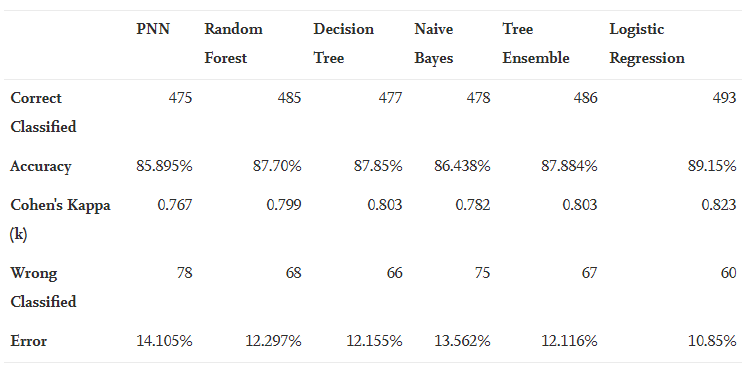
\includegraphics[width=0.8\textwidth]{recursos/ComparacionModelos}
	\label{fig:compResMod}
\end{figure*}
\FloatBarrier

En este artículo \citeA{ADEKITAN2019e01250}, se puede observar como la regresión logística obtiene la mayor precisión en los resultados. Otro artículo donde la regresión logística es la que mejor precisión ofrece es el de \citeA{lehr2016use}, donde además se utilizan los algoritmos de Naïves Bayes, Bosques aleatorios, arboles de decisión y K-vecinos-cercanos.



\section{Herramientas analizadas para la minería de datos}
Existen diversas herramientas para realizar minería de datos, por ello, se debe analizar cuales se utilizan en los artículos estudiados e incluso se debe revisar no solo en el ámbito educativo, sino de forma general. De esta forma obtendremos las herramientas más utilizadas.

En el artículo de \citeA{rodriguez2009herramientas} se recogen algunas de las más utilizadas. Entre ellas se destacan: SPSS Clementine, WEKA y Oracle Data Miner. Además, artículos como el de \citeA{jose2016explotacion} han utilizado R, que es un lenguaje estadístico.

R al estar orientado a la estadística, proporciona un gran número de bibliotecas y herramientas. Destaca también por la generación de gráficos estadísticos de gran calidad. Posee muchos paquetes dedicados a la graficación. Además, es una herramienta que facilita el cálculo numérico y el uso en la minería de datos. \cite{emanuel2014}

Su potencia reside fundamentalmente en que es un software gratuito y de código abierto. Como ya se ha comentado, posee un gran número de herramientas que pueden ampliarse mediante paquetes, librerías o definiendo funciones propias.

Por otro lado, RStudio es el entorno de desarrollo para R. Es también software libre y tiene la ventaja que se puede ejecutar sobre distintas plataformas (Windows, Mac y Linux).

En el artículo de \citeA{jaramillo2015aplicacion}, se ha realizado una breve comparación nuevamente entre las herramientas de WEKA, RapidMiner y Knime. De esta comparación, los autores han seleccionado la herramienta de RapidMiner para realizar las investigaciones por las siguientes características: ``posee una licencia libre, combinación de modelos, interfaz amiga, multiplataforma, empleo de técnicas, además permite aplicar varios algoritmos de minería de datos...'' \cite{jaramillo2015aplicacion}

En la figura \ref{fig:top10tools} se pueden observar las 10 herramientas más utilizadas en 2013 según Rexer Analytics. \cite{rexer2013}

\begin{figure*}[htb]
	\centering
	\caption{Herramientas más usadas. Recuperado de \protect\cite{rexer2013}}
	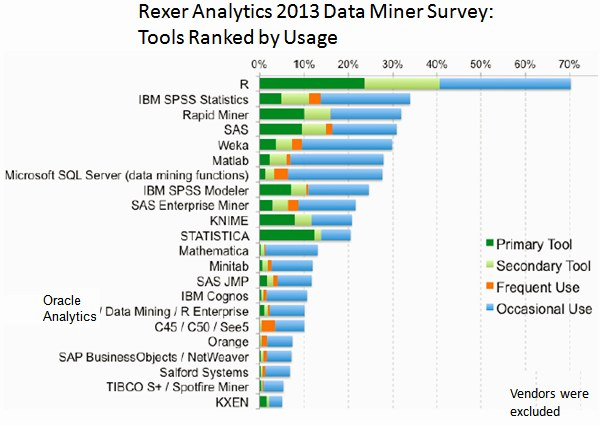
\includegraphics[width=0.8\textwidth]{recursos/top10tools}
	\label{fig:top10tools}
\end{figure*}


Como se puede observar en la figura \ref{fig:top10tools}, las herramientas más utilizadas son R, IBM SPSS Statistics, RapidMiner, y también en puestos superiores se encuentra Weka.

Por otro lado, también se ha consultado la página de Gartner, que es una empresa consultora y de investigación de las tecnologías de la información y que realiza informes sobre las herramientas existentes. En la siguiente figura \ref{fig:gartner} se muestran las herramientas más usadas dividas en cuadrantes dependiendo de la habilidad necesaria para usarlas y la visión completa de estas.

\begin{figure*}[htb]
	\centering
	\caption{Plataformas de ciencia de datos y aprendizaje de máquina. Recuperado de Gartner (https://www.gartner.com)}
	\includegraphics[width=0.6\textwidth]{recursos/gartner}
	\label{fig:gartner}
\end{figure*}


Teniendo conocimiento sobre las herramientas más utilizadas, se debe elegir una de ellas para realizar la investigación de este TFM.

\FloatBarrier

\section{Conclusiones}
%Una vez que se ha realizado un análisis sobre la metodología utilizada y los algoritmos predictivos, además de tener en cuenta las variables utilizadas (relacionadas con el entorno del alumno), se va a realizar una investigación sobre nuevas variables que podrían incluirse en este TFM.

A partir de los artículos anteriores, se observa que existen metodologías, técnicas y herramientas comunes, sin embargo, dependiendo del artículo, unas técnicas obtienen mejores resultados que otras. Esto se debe al carácter de los datos. 

En cuanto a las metodologías, existen muchas investigaciones que utilizan sus propias metodologías en vez de utilizar aquellas de uso frecuente. No obstante, es importante tener claro el procedimiento a seguir.

Por otro lado, también se ha comprobado que existe un gran número de variables comunes de estudio en la mayoría de los artículos. Esto se debe a que la mayoría de los artículos tienen una gran relación, que es investigar acerca de factores que impliquen un mejor rendimiento en los alumnos. Algunas de estas variables se pueden considerar en la investigación de este TFM.

Respecto a los modelos utilizados en ciertos artículos son más precisos que en otros. Esto se debe a los propios datos. Por tanto, en este TFM se realizan pruebas con distintos modelos y se selecciona el que mejor resultados obtenga. Para esta investigación, se deben seleccionar modelos de carácter regresivo.

Por último, en muchos artículos no se referencian las herramientas utilizadas para llevar a cabo la investigación, sin embargo, se ha acudido a otras fuentes para obtener las herramientas con mayor uso. El uso de unas herramientas u otras, no es relevante, puesto que, a día de hoy, la mayoría de las herramientas satisfacen las necesidades de los investigadores, sin embargo, se debe tener en cuenta la licencia comercial, las posibles librerías, etc. que nos puedan o no proporcionar la herramienta.

%Por tanto, una vez que se ha estudiado una metodología de trabajo, y se han observado un gran número de variables relacionadas con los alumnos y con los centros, además de haber agrupado ciertos algoritmos que pueden aportar mayor información sobre los datos educativos, se va a realizar la investigación propia para resolver el problema propio de este TFM.

Por ello, se considera muy oportuno definir, en base a la literatura existente y a los métodos, técnicas, herramientas, etc. más extendidos entre la comunidad científica, una metodología para diseñar esta investigación y unas herramientas para utilizar en dicha metodología y así satisfacer las necesidades dadas.

%manage, education, data mining -> Castilla y Leon
%GIS-Based SWARA and Its Ensemble by RBF and ICA Data-Mining Techniques for Determining Suitability of Existing Schools and Site Selection of New School Buildings
%https://www.maximaformacion.es/blog-dat/como-seleccionar-las-variables-adecuadas-para-tu-modelo/
